\documentclass[aspectratio=1610]{beamer}

\usepackage{polyglossia}
\setdefaultlanguage{czech}

\usepackage{hyperref}

\usepackage{tikz}
\usepackage{amsmath}
\usepackage{biblatex}
\usepackage{minted}
\usepackage{xcolor}

\usetheme{Berlin}

\definecolor{FITBlue}{RGB}{0,115,188}
\definecolor{FITYellow}{RGB}{249,176,0}

\setbeamercolor{structure}{fg=FITBlue}
\setbeamercolor{palette secondary}{bg=FITBlue}
\setbeamercolor{palette tertiary}{fg=white,bg=FITYellow}

% Sources
\addbibresource{sources.bib}

\title{PSI: Jak na laborky}
\author{Klub FIT++}
\date{2026}

\begin{document}

\maketitle

\section{Něco málo na začátek}

\begin{frame}{Motivace}

\begin{itemize}
  \item Málo úložiště - "vzdálený přístup"
  \item Pomalé procesory - více uživatelů na jednom "mainframe"
  \item Multiplayer hry, webové aplikace
  \item Co je to VPN? Jak se doopravdy schovat?
\end{itemize}

\end{frame}

\begin{frame}{Protokoly}

\begin{itemize}
  \item "a.b.c.d:25565" magický text, který určí na jaký MC server se připojím
  \item "play.hypixel.net", funguje místo IP adres
  \item Wi-Fi zadám heslo a vše magicky funguje (kromě eduroam)
  \item Vše funguje na Apple, Samsungu, MikroTiku, Huawei
\end{itemize}

\end{frame}

\begin{frame}{Protokoly}

\begin{itemize}
  \item Domluva mezi výrobci a vývojáři, jak se co dělá
    \begin{itemize}
      \item Jak jsou uspořádané 1/0 co posíláme, jaká je frekvence přenosu...
      \item Jak by měl vypadat postup dekódování/práce s informacemi
      \item Co dělat, když data přijdou poškozená/nesprávná
    \end{itemize}
  \item Backward/Forward kompatibilita
\end{itemize}

\end{frame}

\begin{frame}{Analogie}

\begin{itemize}
  \item Posílání balíčku
    \begin{itemize}
      \item Podpis - od, pro
      \item Obálka - adresa odesílatele, příjemce
      \item Poštovní vůz/letadlo - město odesílatele/příjemce
    \end{itemize}
  \item Zprávu zabalujeme do "balíčků"
  \item V sítích se toto děje vlastně naopak
\end{itemize}

\end{frame}

\begin{frame}{Digitálněji}

\begin{itemize}
  \item dopis předává Alice Bobovi
    \begin{itemize}
      \item dopis se posílá z Prahy do Brna
        \begin{itemize}
          \item jde o odpověď na předchozí korespondenci s předmětem...
          \item text je "ahoj světe"
        \end{itemize}
    \end{itemize}
  \item zaměnte dopis za Email
\end{itemize}

\end{frame}

\begin{frame}{Konečně jak to je v sítích?}

\begin{figure}[h!]
    \centering
    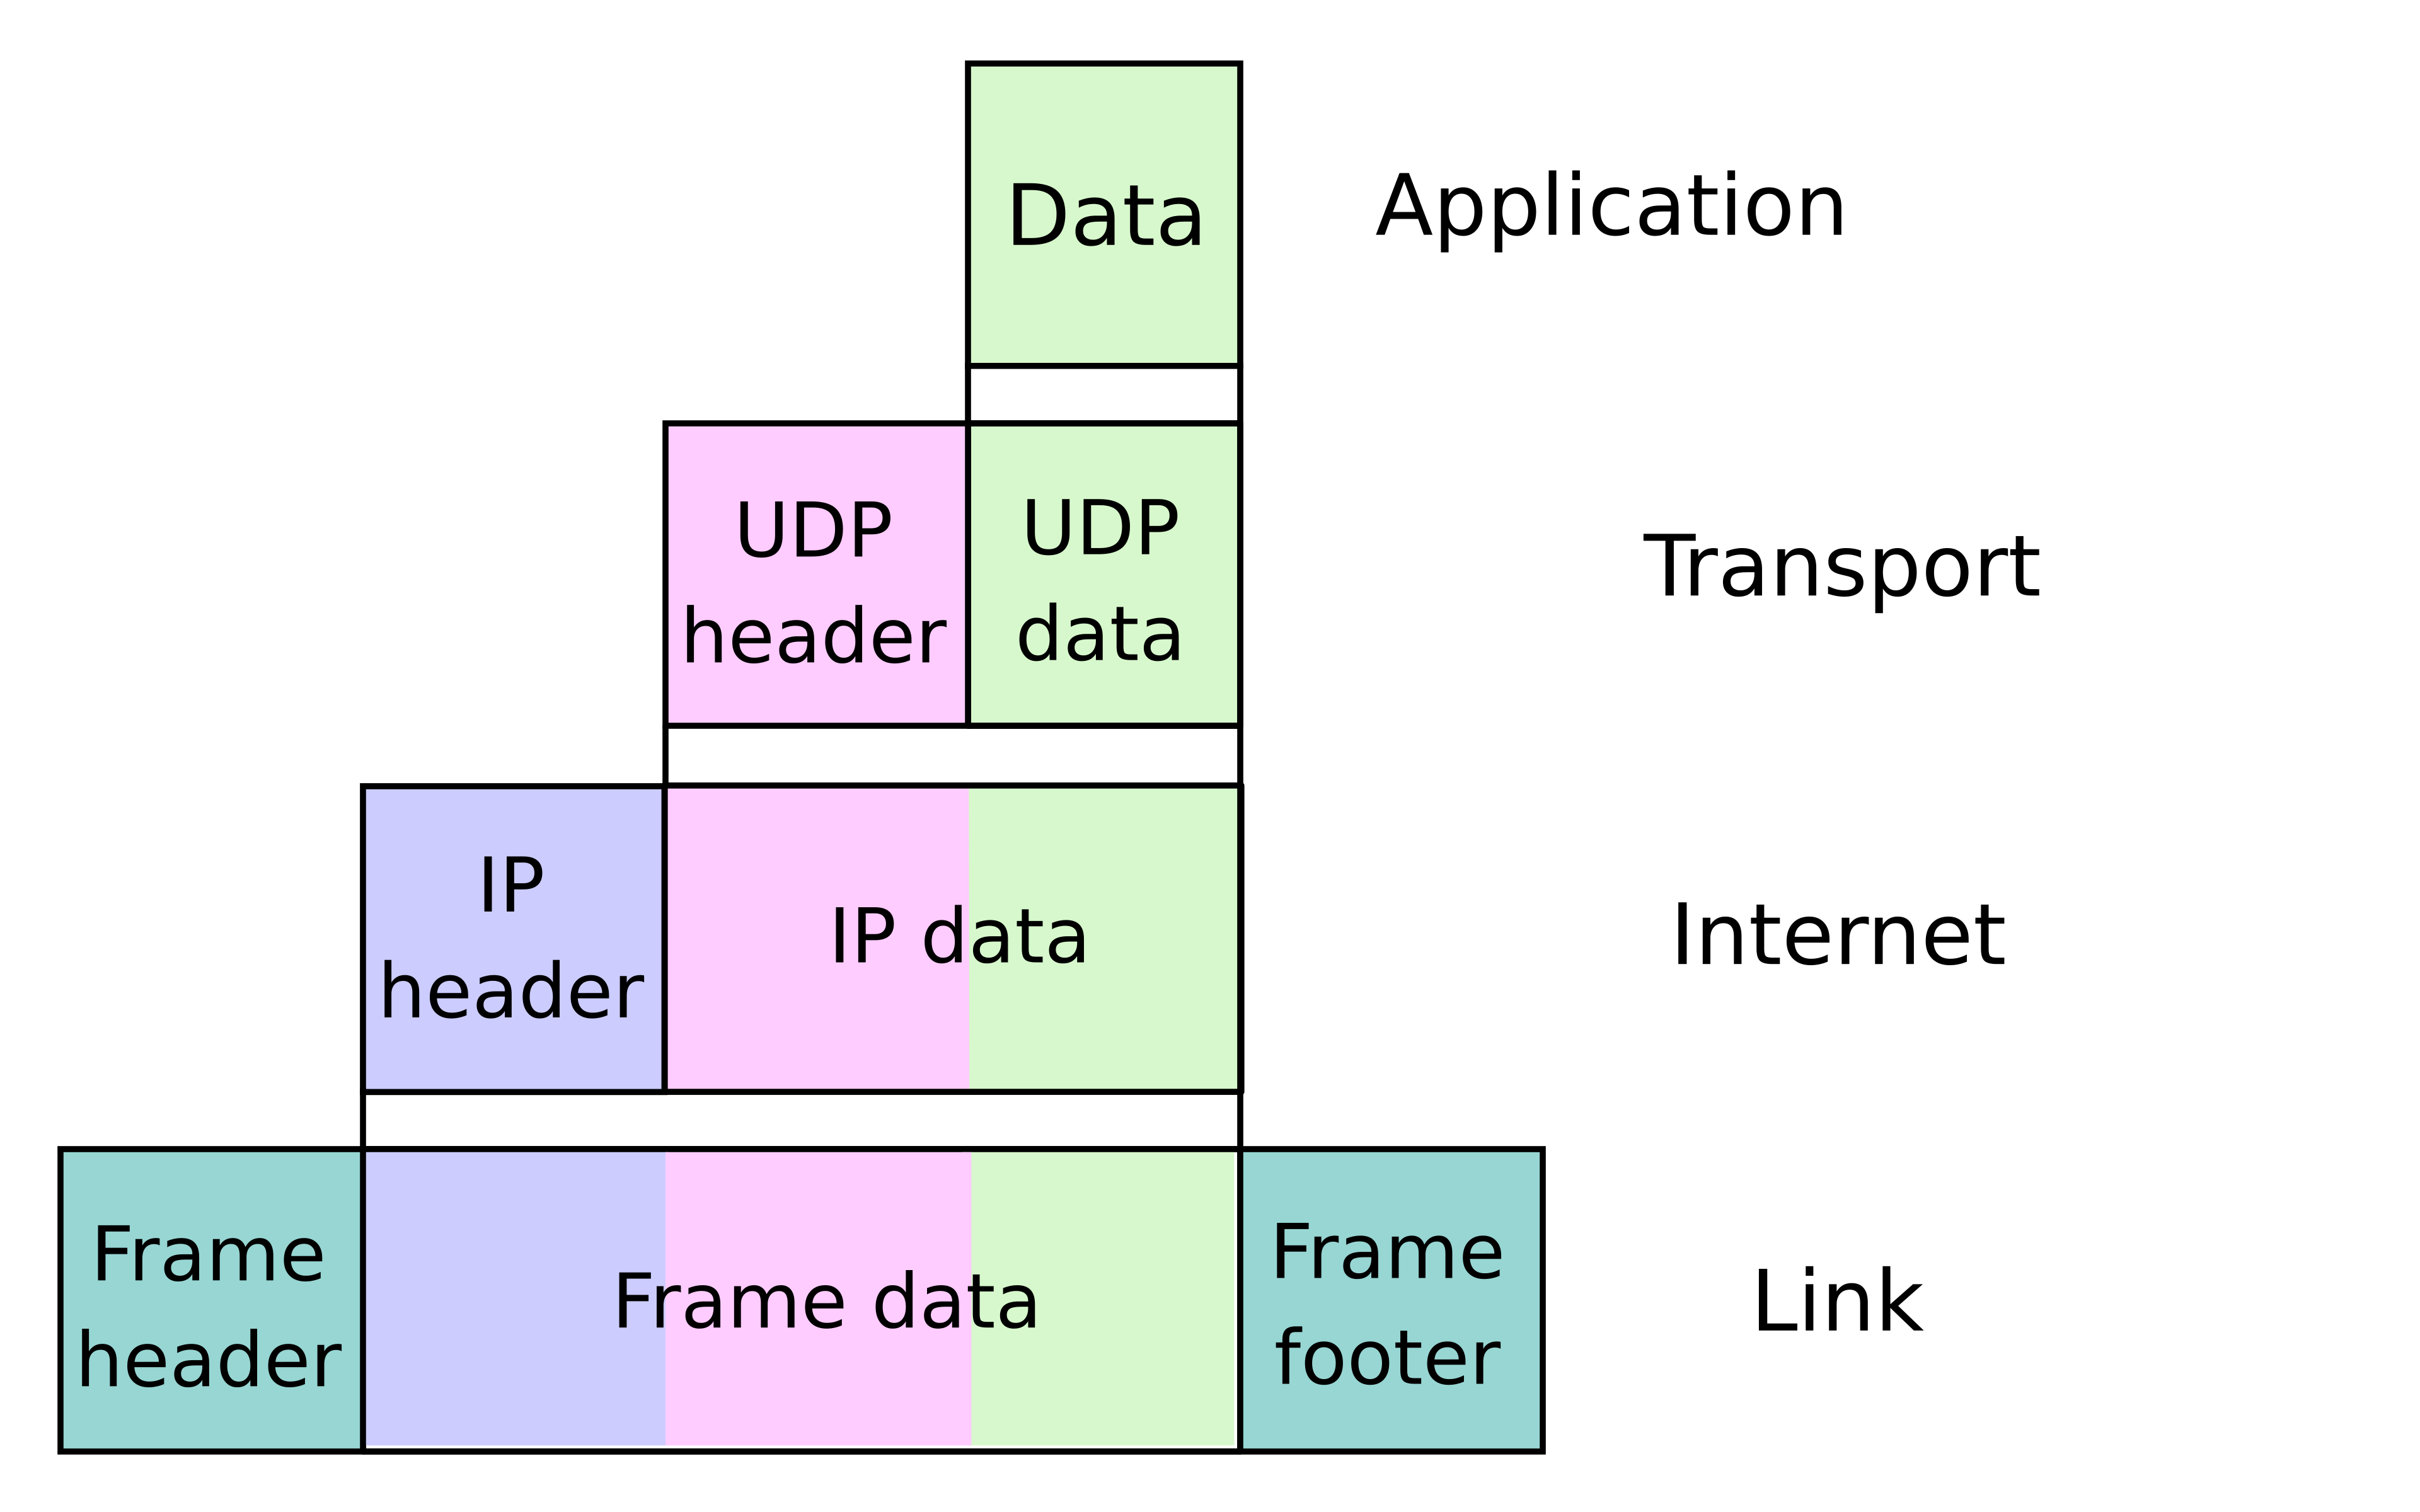
\includegraphics[width=0.6\textwidth]{encapsulation.png}
    \caption{Data jsou schované uvnitř segmentů+packetů+framů (resp. jejich hlavičkách)\cite{wiki:encapsulation}}
\end{figure}

\end{frame}

\begin{frame}{Konečně jak to je v sítích?}

\begin{figure}[h!]
    \centering
    
\includegraphics[width=0.8\textwidth]{frame.png}
    \caption{Ethernetový frame - Na rozeznání, že jde o Ethernet frame hledáme Preamble, co je uvnitř říká Ethertype.\cite{wiki:ethernet}}
\end{figure}

\end{frame}

\section{GNS3 - Instalace a ukázka}

\begin{frame}{Co je GNS3}

\begin{itemize}
  \item Síťový hardware často vypadá jinak než typické počítače
  \item GNS3 je simulátor tohoto hardwaru
  \item Jendnotlivé síťové prvky používají reálný software
  \item Instalace na \href{https://courses.fit.cvut.cz/BI-PSI/labs/tasks_home_study/manuals/manual-gns3.html}{courses}
\end{itemize}

\end{frame}

\begin{frame}{IP adresy, rozsahy}

\begin{itemize}
  \item Jak bylo zmíněno, IPv4 má 4 oktety a.b.c.d
  \item Směrovací identifikátor, používán na 3. vrstvě
  \item Typicky nechceme nastavovat pravidla pro každou IP - proto rozsahy
  \item a.b.c.d/e ($0 \leq e \leq 32$) - kolik bitů se v IP nesmí měnit, aby zůstala v rozsahu (zleva)
\end{itemize}

\end{frame}

\begin{frame}{Spočítání rozsahu}

\begin{itemize}
  \item \texttt{192.168.0.55/24}
  \item \texttt{11000000.10101000.00000000.00110111/24}
  \item \texttt{{\color{red} 11000000.10101000.00000000} 00110111/ {\color{red}24}}
  \item \texttt{{\color{red} 11000000.10101000.00000000} {\color{blue} 00000000}}
  \item \texttt{{\color{red} 11000000.10101000.00000000} {\color{brown} 11111111}}
  \item \texttt{192.168.0.{\color{blue}0} - 192.168.0.{\color{brown}255}}
  \item První a poslední adresa je rezervovaná$^*$
\end{itemize}

\end{frame}

\begin{frame}{Nyní k GNS3}

\centering
\large
Nyní k GNS3

\end{frame}

\begin{frame}{Dotazy}

\centering
\large
Dotazy?

\end{frame}

\printbibliography[title={Zdroje}]

\end{document}
